\chapter{Ionic}\label{ch:ionic}
Al tratarse de un paquete nodeJS, Ionic puede ser instalado usando \gls{npm} de una manera muy sencilla. A continuación detallaremos los pasos a seguir, asumiendo que en la máquina en la que estamos trabajando se encuentra instalado nodeJS y npm (ver anexo).
\begin{itemize}
  \item En primer lugar instalaremos Cordova, usando también para ello \gls{npm}. Para ello ejecutaremos el siguiente comando.
  \begin{lstlisting}[language=bash]
    # npm install -g cordova
  \end{lstlisting}
  El proceso puede tardar unos minutos ya que tendrá que instalar varias dependencias.
  \item Una vez instalado Cordoba, procedemos a la instalación de ionic.
  \begin{lstlisting}[language=bash]
    # npm install -g ionic
  \end{lstlisting}
\end{itemize}

\notebox{Existen dos maneras de instalar paquetes con \gls{npm}, de manera global o de manera local. Si queremos utilizar el paquete como una herramienta vía línea de comandos, debemos instalarla de manera global; en cambio, si queremos que el paquete sea una dependencia del modulo que estamos programando, debemos instalarlo de manera local. La opción \emph{--global/-g} indica a \gls{npm} que el paquete debe ser instalado de manera global ya que por defecto lo instalará de manera local.}

Para probar que se ha instalado de manera correcta, probaremos crearemos un nuevo proyecto y probaremos que funciona.
\begin{itemize}
  \item Dentro de nuestro área de trabajo, crearemos un nuevo proyecto utilizando para ello el comando \emph{ionic start} seguido del nombre de nuestro proyecto.
  \begin{lstlisting}[language=bash]
    # ionic start --v2
  \end{lstlisting}
  \item El anterior comando creará un nuevo directorio con el mismo nombre del proyecto. Dentro de este directorio descargará una templete por defecto, por lo que dentro encontraremos diferentes ficheros y directorios:
  \begin{figure}[H]
\centering
    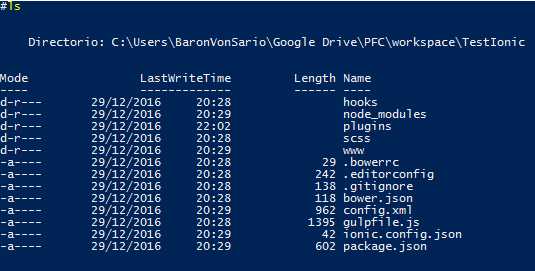
\includegraphics[width=0.8\textwidth]{Figures/anexo/anexoI/ionic/ionic_start}
    \caption{Estructura de archivos que sirve como base para empezar un nuevo proyecto con ionic. Han sido generados utilizando el comando \emph{ionic start}.}
  \end{figure}
  \item Podemos hacer que ionic ponga en marcha un servidor de desarrollo para poder acceder a la aplicación a través de un browser. Solo tenemos que ejecutar el comando \emph{ionic serve} dentro del directorio anterior. Aparecerá un mensaje indicando que el servidor está levantado además de cierta información como la url para acceder a la aplicación, los ficheros que está sirviendo o los comandos para realizar ciertas acciones.
  \begin{figure}[H]
\centering
    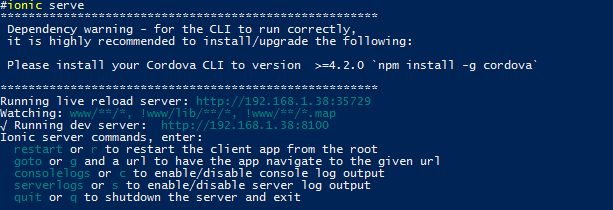
\includegraphics[width=0.8\textwidth]{Figures/anexo/anexoI/ionic/ionic_serve}
    \caption{Vemos como el servidor de la aplicación ionic está en marcha.}
  \end{figure}
  \item Si abrimos nuestro navegador y accedemos a la url que indica el servidor (por defecto será la IP de la máquina y el puerto 8100), veremos la aplicación servida, que no es más que el template descargado anteriormente:
  \begin{figure}[H]
\centering
    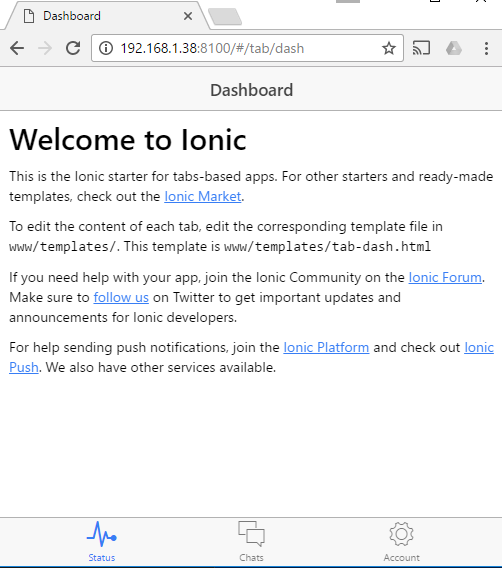
\includegraphics[width=0.8\textwidth]{Figures/anexo/anexoI/ionic/its_alive}
    \caption{La aplicación vista desde un navegador.}
  \end{figure}
\end{itemize}
